%//==============================--@--==============================//%
\subsection{Equações de Maxwell}
\label{subsec:maxwell-eq}

É necessário um conjunto de quatro vetores para descrever os fenómenos do campo eletromagnético:
\begin{itemize}
    \item[] o campo elétrico, $\mathbf{E}$ (unidades: V/m, volt por metro)
    \item[] o campo de indução magnética, $\mathbf{B}$ (unidades: T, tesla)
    \item[] o campo de deslocamento elétrico, $\mathbf{D}$ (unidades: C/m$^2$ , coulomb por metro quadrado)
    \item[] o campo magnético, $\mathbf{H}$ (unidades: A/m, ampère por metro)
\end{itemize}
\noindent Entre estes, os dois primeiros têm significado físico especial, uma vez que podem ser determinados experimentalmente e medidos.

Para fenómenos eletromagnéticos variáveis no tempo consideraram-se as equações de Maxwell:
$$
    \begin{cases}%
        \text{rot } \mathbf{E} = -\dfrac{\partial \mathbf{B}}{\partial t} & \text{\small (Lei de Indução)} \\
        \text{div } \mathbf{D} = \rho & \text{\small (Lei de Gauss)} \\
        \text{rot } \mathbf{H} = \mathbf{J} + \dfrac{\partial \mathbf{D}}{\partial t} & \text{\small (Lei de Ampère com a correção de Maxwell)} \\
        \text{div } \mathbf{B} = 0 & \text{\small (Lei de Gauss para o magnetismo)}
    \end{cases}
$$
em que $\mathbf{D} = \varepsilon \mathbf{E}$ (onde $\varepsilon$ é a permitividade do meio, em F/m), $\mathbf{J} = \sigma \mathbf{E}$ (onde $\sigma$ é a condutividade do condutor, em S/m) e $\mathbf{B} = \mu \mathbf{H}$ (onde $\mu$ representa a permeabilidade do meio, em H/m).

%//==============================--@--==============================//%
\subsection{Circuitos Magnéticos}
\label{subsec:circuitos-magneticos}

É importante revisitar os conceitos fundamentais dos circuitos magnéticos: 
$$
    \begin{aligned}
        \text{\underline{Tensão magnética}: }& u_m \delequal \int_C \mathbf{H} \cdot d\mathbf{r} \\
        \text{\underline{Fluxo magnético}: }& \Phi_m \delequal \int\!\!\int_S \mathbf{B} \cdot \mathbf{n}\; dS\\
        \text{\underline{Relutância magnética}: }& R_m \delequal \frac{u_m}{\Phi_m}
    \end{aligned}
$$
Salienta-se que o fluxo magnético obedece à \textit{Lei dos Cortes} --- análoga ao KCL --- uma vez que $\text{div } \mathbf{B} = 0$, temos que $\sum_i^n \Phi_{m_i} = 0$ numa superfície fechada (ou ``nó''); enquanto, em geral, a tensão magnética \textbf{não} obedece a nenhuma lei semelhante ao KVL.

\vspace{0.5em}
\noindent As \hyperref[subsec:maxwell-eq]{equações de Maxwell acima} condensam duas leis essenciais a este capítulo:
\begin{enumerate}
    \item[] \textbf{Lei de Indução}: A expressão <<$\text{rot } \mathbf{E} = -\partial \mathbf{B}/\partial t$>> diz que um campo magnético que varia com o tempo é sempre acompanhado por um campo elétrico não-conservativo que varia espacialmente, e vice-versa.
    $$
        \iint_{S_N} \text{rot } \mathbf{E} \cdot \mathbf{n}\, dS = -\iint_{S_N} \dfrac{\partial \mathbf{B}}{\partial t} \cdot \mathbf{n}\, dS \iff \oint_{\partial S_N} \mathbf{E} \cdot d\mathbf{r} = -\dfrac{d}{dt} \iint_{S_N} \mathbf{B} \cdot \mathbf{n}\, dS 
    $$
    $$
        \boxed{ \therefore \text{e.m.f.} = -\frac{d \Psi}{dt} = -N\frac{d \Phi_m}{dt} }
    $$
    em que $\Psi = N\Phi_m$ é definido como o \textit{fluxo magnético ligado}.

    \item[] \textbf{Lei de Ampère}: A expressão <<$\text{rot } \mathbf{H} = \mathbf{J} + \partial \mathbf{D}/\partial t$>> afirma que campos magnéticos podem ser criados de duas formas: através de correntes elétricas, que é a lei de Ampère original, e por campos elétricos que variam no tempo, que é a correção proposta por Maxwell (nesta UC não consideramos este fenómeno).
    $$
        \iint_{S_N} \text{rot } \mathbf{H} \cdot \mathbf{n}\, dS = \iint_{S_N} \mathbf{J} \cdot \mathbf{n}\, dS \iff \oint_{\partial S_N} \mathbf{H} \cdot d\mathbf{r} = I_{\partial S} = N I > 0 \text{ (quando $\mathbf{H}$ é concordante com $d\mathbf{r}$)}
    $$
\end{enumerate}

\noindent O fluxo ligado é uma quantidade proporcional à corrente --- de onde se define o coeficiente de indução,
$$
    \Psi = N \Phi = \iint_{S_N} \mathbf{B} \cdot \mathbf{n}\, dS = L I
$$

\renewcommand{\thefootnote}{\fnsymbol{footnote}}
\footnotetext[4]{%
    A constante $N$ representa, naturalmente, o número de espiras do enrolamento em questão.
}
\renewcommand{\thefootnote}{\arabic{footnote}}

%//==============================--@--==============================//%
\subsection{Transformador}
\label{subsec:transformador}

%//==============================--@--==============================//%
\subsubsection{Funcionamento do Transformador}
\label{subsec:transformador-funcionamento}

%//==============================--@--==============================//%
\paragraph{Transformador Ideal}
\label{subsubsec:transformador-ideal}

Para o transformador monofásico ideal assumimos duas aproximações: enrolamentos com resistência nula e circuito magnético com relutância igualmente nula (isto implica que não existe dispersão).

\vspace{-0.75em}
\begin{minipage}[c]{0.35\linewidth}
    \begin{figure}[H]
        \centering
        \begin{circuitikz}[>=stealth, scale=0.9, american]
            \draw (0,0) node[transformer] (T) {};
            \draw (T.A1) -- ++(-1,0) node[circ] {};
            \draw (T.A2) -- ++(-1,0) node[circ] {};
            \draw (T.B1) -- ++(1,0) node[circ] {};
            \draw (T.B2) -- ++(1,0) node[circ] {};
    
            \node[left=4.5mm,above=4mm] at (T.outer dot A2) {$N_1$};
            \node[right=4.5mm,above=4mm] at (T.outer dot B2) {$N_2$};
    
            \node[draw,dotted,fit=(T.inner dot A1)(T.inner dot A2)(T.inner dot B1)(T.inner dot B2),inner sep=1.25mm] (dottedrect) {};
            
            \node[above] at (dottedrect.north) {$\Phi$};
            \draw[->] (dottedrect.north) -- ++(0.075,0);
    
            % voltage drops
            \draw[->] ([xshift=-1cm, yshift=-1.5mm]T.A1) -- ([xshift=-1cm, yshift=+1.5mm]T.A2) node[midway,left] {$v_1$};
            \draw[->] ([xshift=+1cm, yshift=-1.5mm]T.B1) -- ([xshift=+1cm, yshift=+1.5mm]T.B2) node[midway,right] {$v_2$};
    
            % currents
            \draw[->] ([xshift=-0.50cm]T.A1) -- ([xshift=-0.05cm]T.A1) node[above] {$i_1$};
            \draw[->] (T.B1) -- ([xshift=+0.25cm]T.B1) node[above] {$i_2$};

            % add transformer dots
            \node[circ,scale=0.75,yshift=-2.75mm] at (T.outer dot A1) {};
            \node[circ,scale=0.75,yshift=-2.75mm] at (T.outer dot B1) {};
        \end{circuitikz}
        \caption{Transformador ideal.}
        \label{fig:ideal-transformer}
    \end{figure}
\end{minipage}
\begin{minipage}[c]{0.6\linewidth}
    \noindent Neste primeiro modelo temos as seguintes relações:
    $$
        \begin{dcases}
            v_1 = N_1 \frac{d \Phi}{dt}\\
            v_2 = N_2 \frac{d \Phi}{dt}
        \end{dcases}
        \implies
        \begin{dcases}
            \mathbf{V}_1 = j\omega N_1 \Phi \\
            \mathbf{V}_2 = j\omega N_2 \Phi
        \end{dcases}
        \implies \frac{\mathbf{V}_1}{\mathbf{V}_2} = \frac{V_1}{V_2} = \frac{N_1}{N_2}
    $$
\end{minipage}

\vspace{0.75em}
\noindent Uma vez que a resistência dos enrolamentos é nula e a reatância de dispersão também é nula, \underline{não há perdas} de potência ativa nem de potência reativa. \underline{A potência complexa é igual nos dois lados} do transformador:
$$
    \mathbf{S}_1 = \mathbf{S}_2 \iff \mathbf{V}_1 \mathbf{I}_1^* = \mathbf{V}_2 \mathbf{I}_2^* \implies \frac{\mathbf{I}_1}{\mathbf{I}_2} = \frac{I_1}{I_2} = \frac{N_2}{N_1}
$$
É útil definir a relação de transformação $m$, o quociente entre o número de espiras do primário (enrolamento que recebe energia) e do secundário (enrolamento que cede energia):
$$
    m = \frac{\mathbf{V}_1}{\mathbf{V}_2} = \frac{N_1}{N_2} = \frac{V_{n1}}{V_{n2}} \; \text{kV/kV}
$$
onde $V_{n1}$ é a tensão nominal primária e $V_{n2}$ a tensão nominal secundária.

\renewcommand{\thefootnote}{\fnsymbol{footnote}}
\footnotetext[4]{%
    A tensão nominal, também conhecida como tensão nominal de operação, é um valor específico de tensão elétrica que um equipamento, dispositivo ou sistema elétrico é projetado para operar de forma ideal e segura.
}
\renewcommand{\thefootnote}{\arabic{footnote}}

%//==============================--@--==============================//%
\paragraph{Não Idealidades do Transformador e Corrente de Magnetização}
\label{subsubsec:corrente-magnetizacao}

O núcleo do transformador é normalmente constituído por ferro, que possui uma característica B-H não linear: a partir de um certo valor dos campos manifesta-se saturação. Acresce-se ainda o fenómeno da histerese, i.e., as trajetórias B-H são distintas para valores crescentes ou decrescente do campo magnético.

\begin{minipage}[b]{0.275\linewidth}
   \begin{figure}[H]
        \centering
        \scalebox{0.6}{%
            \begin{tikzpicture}
                \begin{axis}[very thick,
                             samples = 100,
                             xlabel = H,
                             ylabel = B,
                             xmin = -6,
                             xmax = 6,
                             ymin = -4,
                             ymax = 4,
                             axis x line = middle,
                             axis y line = middle,
                             ticks = none]
                    \addplot[dashed] plot (\x, 2.5);
                    \addplot[dashed] plot (\x,-2.5);
                    \addplot[red, name path=A] plot (\x, {5/(1 + exp(-1.7*\x+1.5))-2.5});
                    \addplot[red, name path=B] plot (\x, {5/(1 + exp(-1.7*\x-1.5))-2.5});
                    \addplot[red!20] fill between[of=A and B];
                \end{axis}
            \end{tikzpicture}
        }
        \caption{Característica magnética do núcleo do transformador}
        \label{fig:hysteresis-iron}
    \end{figure} 
\end{minipage}\hfill
\begin{minipage}[b]{0.65\linewidth}
    O ponto de funcionamento na curva B-H está normalmente localizado próximo ao cotovelo que marca o início da saturação.

    \hspace{1em} O fluxo magnético alternado dá origem a perdas no núcleo de ferro devidas à histerese e às correntes de fuga. ``As primeiras resultam da energia necessária para orientar os domínios magnéticos do material na direção do campo; as segundas devem-se ao efeito de Joule resultante das correntes induzidas no ferro''\cite{paiva2005}.

    \hspace{1em} Uma vez que a permeabilidade do ferro não é infinita, a relutância do circuito magnético não é nula. Introduz-se a \textit{corrente de magnetização} necessária para criar o campo magnético $\mathbf{H}$, fornecida pela rede/gerador que alimenta o transformador.
\end{minipage}

\vspace{0.75em}
\noindent A componente fundamental da corrente de magnetização, à frequência nominal, pode medir-se através de um ensaio em vazio do transformador (que \hyperref[subsec:analise-transformador]{veremos em seguida}).

O esquema equivalente representa-se na \hyperref[fig:esquema-equiv-transformador]{Fig. 12}: as componentes em fase e em quadratura da corrente de magnetização circulam através da condutância $G_m$ e suscetância $B_m$, respetivamente. A componente transversal do esquema equivalente, pertence à modelação da corrente de magnetização. As componentes das impedâncias longitudinais são devido à resistência dos condutores e à reatância de dispersão. 

\vspace{-0.5em}
\begin{theo}[Perdas no Transformador]{def:perdas-transformador}
    Cumulativamente, podemos calcular as perdas no transformador conforme a diferença
    $$
        \text{Perdas} = P_1 - P_2 = P_{cu} + P_{fe}
    $$
    em que $P_1$ e $P_2$ representam a potência ativa no primário e no secundário, respetivamente. A distribuição destas perdas corresponde à contribuição do circuito elétrico (nos enrolamentos de cobre) e do circuito magnético (no núcleo de ferro):
    $$
        P_{cu} = R_1 I_1^2 + R_2 I_2^2 \simeq R_t I_2^2 \quad\land\quad P_{fe} \simeq G_m V_1^2
    $$
\end{theo}

%//==============================--@--==============================//%
\clearpage
\paragraph{Esquema Equivalente do Transformador}
\label{subsubsec:equiv-esquema}

Um primeiro esquema equivalente do transformador pode ser dado por:

\begin{figure}[H]
\centering
    %\resizebox{0.8\textwidth}{!}{%
    \ctikzset{bipoles/resistor/height=0.20}
    \ctikzset{bipoles/resistor/width=0.5}
        \begin{circuitikz}[>=stealth,american,scale=0.95]
            
            % Resistor
            \draw (2,0) to[R] (4,0);
            \node at (3,0.4) {$R_1$};
            
            \draw (5.5,-1) to[R] (5.5, -2);
            \node at (5,-1.5) {$G_m$};
            
            \draw (9,0) to[R] (11, 0);
            \node at (10,0.4) {$R_2$};
            
            % Inductor
            \draw (4,0) to[cute inductor] (6,0);
            \node at (5,0.5) {$jX_1$};
            
            \draw (8,0) to[cute inductor] (8,-3);
            \draw (9,-3) to[cute inductor] (9,0);
            
            \draw (6.5,-1) to[cute inductor] (6.5,-2);
            \node at (7.15,-1.5) {$jB_m$};
            
            \draw (11,0) to[cute inductor, -*] (13,0);
            \node at (12,0.5) {$jX_2$};
            
            % Wires
            \draw (6,0) to[short, *-] (8, 0);
            \draw (5.5,-0.5) to[short, -] (6.5, -0.5);
            \draw (5.5,-2.5) to[short, -] (6.5, -2.5);
            \draw (5.5,-1) to[short, -] (5.5, -0.5);
            \draw (6.5,-1) to[short, -] (6.5, -0.5);
            \draw (5.5,-2) to[short, -] (5.5, -2.5);
            \draw (6.5,-2) to[short, -] (6.5, -2.5);
            \draw (6,0) to[short, *-] (6, -0.5);
            \draw (6,-3) to[short, *-] (6, -2.5);
            \draw (6,-3) to[short, -] (8, -3);
            \draw (1,-3) to[short, *-] (6, -3);
            \draw (9,-3) to[short, -*] (13, -3);
            
            % Nodes
            \draw (2, 0) to[short, -*] (1,0);
            \draw (6,0) to[short, -*] (6,0);
            \draw [fill=black] (7.87, -1.1)node(a){} circle (1pt);
            \draw [fill=black] (9.13, -1.1)node(a){} circle (1pt);
            
            % Arrows
            \draw[->,thick](1, -0.2) to[short] (1,-2.8);
            \node at (0.7,-1.5) {$V_1$};
            
            \draw[->,thick](13, -0.2) to[short] (13,-2.8);
            \node at (13.3, -1.5) {$V_2$};
            
            \draw[->,thick](9.3, -0.4) to[short] (9.3,-2.6) node[right] {$E_2$};
            \draw[->,thick](7.7, -0.4) to[short] (7.7,-2.6) node[left] {$E_1$};
            
            \draw[->,thick](1.7, 0) to[short] (1.8,0) node[above] {$I_1$};
            \draw[->,thick](7, 0) to[short] (7.1,0) node[above] {$I_2'$};
            \draw[->,thick](12.6, 0) to[short] (12.7,0) node[above] {$I_2$};
            \draw[->,thick](6, -0.3) to[short] (6,-0.4);
            \node at (6.3, -0.25) {$I_m$};
            
        \end{circuitikz}
    %}%
    
    \caption{Esquema Equivalente do transformador.}
    \label{fig:esquema-equiv-transformador}
\end{figure}
\vspace{-1em}
$$
    \left\{\begin{aligned}
        E_1 &= V_1 -  \left(RI_1 + jX_1I_1\right)\\
        E_2 &= V_2 +  RI_2 + jX_2I_2
    \end{aligned}\right.\qquad
    \left\{\begin{aligned}
        I_1 &= I_m + I_2'\\
        I_2' &= \frac{N_2}{N_1} I_2
    \end{aligned}\right.   
$$
Se tomarmos as tensões de base, do lado do primário e do secundário, pelas respetivas tensões nominais, i.e., $V_{b1} = V_{n1}$ e $V_{b2} = V_{n2}$, a relação do transformador em valores p.u. é
$$
    m = \frac{V_{{n1}_{pu}}}{V_{{n2}_{pu}}} = \frac{V_{n1}}{V_{b1}} \frac{V_{b2}}{V_{n2}} = 1.0\; \text{p.u.}
$$
Esta conclusão indica que o transformador ideal \underline{pode ser removido do esquema equivalente} da rede, uma vez que a relação de transformação é unitária. 

Chegamos assim ao esquema equivalente em T:
\begin{figure}[H]
    \centering
    %\resizebox{0.65\textwidth}{!}{%
    \ctikzset{bipoles/resistor/height=0.20}
    \ctikzset{bipoles/resistor/width=0.5}
        \begin{circuitikz}[>=stealth,american,scale=0.95]
            
            % Resistor
            \draw (2,0) to[R] (4,0);
            \node at (3,0.4) {$R_1$};
            
            \draw (5.5,-1) to[R] (5.5, -2);
            \node at (5,-1.5) {$G_m$};
            
            \draw (6,0) to[R] (8, 0);
            \node at (7,0.4) {$R_2$};
            
            % Inductor
            \draw (4,0) to[cute inductor] (6,0);
            \node at (5,0.5) {$jX_1$};
            
            \draw (6.5,-1) to[cute inductor] (6.5,-2);
            \node at (7.15,-1.5) {$jB_m$};
            
            \draw (8,0) to[cute inductor, -*] (10,0);
            \node at (9,0.5) {$jX_2$};
            
            % Wires
            \draw (5.5,-0.5) to[short, -] (6.5, -0.5);
            \draw (5.5,-2.5) to[short, -] (6.5, -2.5);
            \draw (5.5,-1) to[short, -] (5.5, -0.5);
            \draw (6.5,-1) to[short, -] (6.5, -0.5);
            \draw (5.5,-2) to[short, -] (5.5, -2.5);
            \draw (6.5,-2) to[short, -] (6.5, -2.5);
            \draw (6,0) to[short, *-] (6, -0.5);
            \draw (6,-3) to[short, *-] (6, -2.5);
            \draw (1,-3) to[short, *-] (6, -3);
            \draw (6,-3) to[short, -*] (10, -3);
            
            % Nodes
            \draw (2, 0) to[short, -*] (1,0);
            \draw (6,0) to[short, -*] (6,0);
        
            
            % Arrows
            \draw[->,thick](1, -0.2) to[short] (1,-2.8);
            \node at (0.7,-1.5) {$V_1$};
            
            \draw[->,thick](10, -0.2) to[short] (10,-2.8);
            \node at (10.3, -1.5) {$V_2$};
            
            \draw[->,thick](1.7, 0) to[short] (1.8,0) node[above] {$I_1$};
            \draw[->,thick](9.6, 0) to[short] (9.7,0) node[above] {$I_2$};
            \draw[->,thick](6, -0.3) to[short] (6,-0.4);
            \node at (6.3, -0.25) {$I_m$};
            
        \end{circuitikz}
    %}%
    
    \caption{Esquema Equivalente em T do transformador.}
\end{figure}

\noindent O fluxo no núcleo mantém-se constante pelo que as admitâncias do ramo transversal que modelam a corrente de magnetização se podem considerar constantes. \underline{A corrente de magnetização é pequena} (alternativamente, a impedância do ramo transversal é muito maior que impedância longitudinal dos dois lado), logo, o ramo transversal pode ser levado para um dos extremos, resultando no esquema em L:
\begin{figure}[H]
    \centering
    %\resizebox{0.55\textwidth}{!}{%
    \ctikzset{bipoles/resistor/height=0.20}
    \ctikzset{bipoles/resistor/width=0.5}
        \begin{circuitikz}[>=stealth,american,scale=0.95]
            
            % Resistor
            \draw (5.5,-1) to[R] (5.5, -2);
            \node at (5,-1.5) {$G_m$};
            
            \draw (6,0) to[R] (8, 0);
            \node at (7,0.4) {$R_t$};
            
            % Inductor
            \draw (6.5,-1) to[cute inductor] (6.5,-2);
            \node at (7.15,-1.5) {$jB_m$};
            
            \draw (8,0) to[cute inductor, -*] (10,0);
            \node at (9,0.5) {$jX_t$};
            
            % Wires
            \draw (5.5,-0.5) to[short, -] (6.5, -0.5);
            \draw (5.5,-2.5) to[short, -] (6.5, -2.5);
            \draw (5.5,-1) to[short, -] (5.5, -0.5);
            \draw (6.5,-1) to[short, -] (6.5, -0.5);
            \draw (5.5,-2) to[short, -] (5.5, -2.5);
            \draw (6.5,-2) to[short, -] (6.5, -2.5);
            \draw (6,0) to[short, *-] (6, -0.5);
            \draw (6,-3) to[short, *-] (6, -2.5);
            \draw (3,-3) to[short, *-] (6, -3);
            \draw (6,-3) to[short, -*] (10, -3);
            
            % Nodes
            \draw (6, 0) to[short, -*] (3,0);
            \draw (6,0) to[short, -*] (6,0);
        
            
            % Arrows
            \draw[->,thick](3, -0.2) to[short] (3,-2.8);
            \node at (2.7,-1.5) {$V_1$};
            
            \draw[->,thick](10, -0.2) to[short] (10,-2.8);
            \node at (10.3, -1.5) {$V_2$};
            
            \draw[->,thick](3.7, 0) to[short] (3.8,0) node[above] {$I_1$};
            \draw[->,thick](9.6, 0) to[short] (9.7,0) node[above] {$I_2$};
            \draw[->,thick](6, -0.3) to[short] (6,-0.4);
            \node at (6.3, -0.25) {$I_m$};
            
        \end{circuitikz}
    %}%
    
    \caption{Esquema Equivalente em L do transformador.}
\end{figure}
$$
    \left\{\begin{aligned}
        R_t &= R_1 + R_2\\
        X_t &= X_1 + X_2
    \end{aligned}\right.\qquad
    Z_t = R_t + jX_t
$$

%//==============================--@--==============================//%
\subsubsection{Análise do Transformador}
\label{subsec:analise-transformador}
%//==============================--@--==============================//%
\paragraph{Ensaio em Vazio}
Aplica-se a tensão nominal ao enrolamento que produz a menor corrente de magnetização, e o outro enrolamento em aberto.

\begin{figure}[H]
    \centering
    \ctikzset{bipoles/resistor/height=0.20}
    \ctikzset{bipoles/resistor/width=0.5}
    \begin{circuitikz}[=>stealth,american]
        % circuito
        \draw (0,0) to [short, *-] (3,0);

        \draw (3,-0.5) to [short] (3,0);
        \draw (2.5,-0.5) to [short] (3.5,-0.5);
        \draw (2.5,-0.5) to [R, l_=$G_m$] (2.5,-2.5);
        \draw (3.5,-0.5) to [cute inductor, l=$jB_m$] (3.5,-2.5);
        \draw (2.5,-2.5) to [short] (3.5,-2.5);
        \draw (3,-2.5) to [short] (3,-3);

        \draw (3,-3) to [short] (0,-3) node[circ] {};

        % tensão e corrente de magnetização
        \draw[->] (0,-0.25) -- (0,-2.75) node[midway,left] {$V_n$};
        \draw[->] (3,-0.25) -- (3,-0.30) node[midway,right] {$I_m$};
    \end{circuitikz}
    \caption{Transformador com o secundário em aberto.}
    \label{fig:ensaio-vazio-transformador}
\end{figure}

\noindent Os valores de $G_m$ e $B_m$ obtêm-se através das medidas da tensão aplicada $V_n$, corrente de magnetização $I_m$ e potência de perdas em vazio $P_0$:
$$
    G_m = \frac{P_0}{V_n^2} 
    \mkern48mu
    B_m = -\sqrt{\left(\frac{I_m}{V_n}\right)^2-G_m^2}
$$
\textbf{Nota:} A suscetância $B_m$ é negativa de forma a que a reatância respetiva seja indutiva.
%//==============================--@--==============================//%
\paragraph{Ensaio em Curto-Circuito}

\noindent Através de um ensaio em curto-circuito do transformador pode medir-se o módulo da impedância de $Z_t$ (normalmente designada por impedância de curto circuito $Z_{cc}$). Aplica-se um curto circuito a um dos enrolamentos e alimenta-se o outro com uma tensão reduzida (tensão de curto-circuito $V_{cc}$), de modo a que a corrente fique no seu valor nominal (de modo a não fritar o circuito).

\begin{figure}[H]
    \centering
    \begin{circuitikz}[>=stealth, scale=0.95]
        % Inductor
        \draw (0,0) to[R] (6,0);
        \node at (3,0.5) {$Z_t = Z_{cc}$};
        
        % Nodes
        \draw (0, 0) to[short, -*] (0,0);
        \draw (0,-2) to[short, -*] (0,-2);
        
        % Wire
        \draw (0, -2) to[short, -] (6,-2);
        \draw (6, 0) to[short, -] (6, -2);
        
        % Arrows
        \draw[->,thick](0, -0.2) to[short] (0,-1.8);
        \node at (-0.3,-1) {$V_{cc}$};
        
        \draw[->,thick](0.5, 0) to[short] (0.55,0) node[above] {$I_n$};
    \end{circuitikz}
    \caption{Transformador em curto-circuito.}
    \label{fig:ensaio-cc-transformador}
\end{figure}

\vspace{-1em}
\noindent\textbf{Nota:} O paralelo de duas resistências é aproximadamente a mais pequena. Como o ramo transversal possui uma impedância muito elevada, \underline{é possível desprezar o ramo e a respetiva corrente de magnetização}. %adoro-te mimo 
$$
    \left\{\begin{aligned}
        V_{cc} &= Z_{cc} I_n\\
        I_n &= 1.0\; \text{p.u.}
    \end{aligned}\right.\quad\rightarrow\quad
    \boxed{V_{cc} = Z_{cc}} 
$$
\noindent Para decompor a impedância de curto-circuito nas suas componentes resistiva e reativa, é preciso conhecer a potência $P_{cc}$:
$$
    R_t = \dfrac{P_{cc}}{I_n^2} = P_{cc}\qquad
    Z_{cc} = V_{cc} = \sqrt{R_t^2 + X_t^2}\qquad
    X_t = \sqrt{Z_t^2 - R_t^2}
$$

\begin{figure}[H]
    \centering
    \scalebox{0.925}{%
        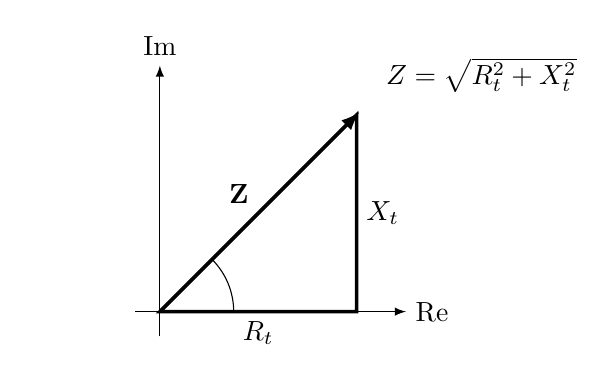
\begin{tikzpicture}[scale=1.25, >=latex]
            % Draw real and imaginary axes
            \draw[->] (-0.25,0) -- (2.5,0) node[right] {Re};
            \draw[->] (0,-0.25) -- (0,2.5) node[above] {Im};
            
            \draw [line width=1.25pt] (0,0) -- (2,0) -- (2,2) -- cycle;
        
            \draw [->, line width=1.25pt] (0,0) -- (2.025,2.025);
            
            \node[below] at (1,0) {$R_t$};
            \node[right] at (2,1) {$X_t$};
            \node[above left] at (1,1) {$\mathbf{Z}$};
            \node[right] at (2.2,2.4) {$Z = \sqrt{R_t^2 + X_t^2}$};
            \node[left] at (-1.15,2) {};
        
            \draw (0.75,0) arc (0:45:0.75); 
        \end{tikzpicture}
    }
    \caption{Decomposição da impedância total equivalente.}
\end{figure}

%//==============================--@--==============================//%
\subsubsection{Configurações Especiais do Transformador}
\label{subsec:transformador-config-especiais}

%//==============================--@--==============================//%
\paragraph{Transformador com Três Enrolamentos}

Trata-se de um transformador com três enrolamentos à volta do mesmo núcleo como se representa na \hyperref[fig:transformador-3-enrolamentos]{Fig. 18}.

\begin{figure}[H]
    \centering
    \scalebox{0.725}{%
    \begin{circuitikz}[american]
        %% Configure circuitikz
        \ctikzset{inductor=cute}    
        \ctikzset{inductors/coils=4}
        \ctikzset{bipoles/resistor/height=0.25}
        \ctikzset{bipoles/resistor/width=0.5}
        \ctikzset{resistors/zigs=4}
    
        %% circuit
        \draw (0,0) to[short,*-] (1,0) to[generic,l^=$Z_1$,-*] (4,0);
        \draw (4,0) to[generic,l^=$Z_2$] (6,2) to[short,-*] (8,2);
        \draw (4,0) to[generic,l^=$Z_3$] (6,-2) to[short,-*] (7,-2);
        \draw (0,-4) to[short,*-*] (8,-4);

        %% optional
        \draw[gray] (4,0) to[short,*-] (4,-1.5) to[short] (3.5,-1.5) to[short] (4.5,-1.5);
        \draw[gray] (3.5,-1.5) to[R,l_=$G_m$] (3.5,-3);
        \draw[gray] (4.5,-1.5) to[L,l=$jB_m$] (4.5,-3);
        \draw[gray] (3.5,-3) to[short] (4.5,-3);
        \draw[gray] (4,-3) to[short,-*] (4,-4);

        %% labels and arrows
        \draw[->,>=stealth] (0,-0.25) -- (0,-3.75) node[midway,left] {$\mathbf{V}_1$};
        \draw[->,>=stealth] (7,-2.25) -- (7,-3.75) node[midway,left] {$\mathbf{V}_3$};
        \draw[->,>=stealth] (8,1.75) -- (8,-3.75) node[midway,right] {$\mathbf{V}_2$};
    \end{circuitikz}}

    \caption{Transformador com três enrolamentos.}
    \label{fig:transformador-3-enrolamentos}
\end{figure}

\vspace{-0.25em}
\noindent No caso de se pretender representar a admitância de magnetização, liga-se entre o nó fictício e o neutro.

As impedâncias do sistemas monofásico equivalente, podem ser obtidas através de três ensaios de curto-circuito (primário-secundário, primário-terciário e secundário-terciário), nos quais se medem $Z_{12}$, $Z_{13}$ e $Z_{23}$, respetivamente:
$$
    \begin{cases}
        Z_{12} = Z_1 + Z_2\\
        Z_{13} = Z_1 + Z_3\\
        Z_{23} = Z_2 + Z_3
    \end{cases}
$$
De onde resulta que
$$
    \left\{
    \begin{aligned}
        Z_1 &= \frac{Z_{12} + Z_{13} - Z_{23}}{2} \\
        Z_2 &= \frac{Z_{12} + Z_{23} - Z_{13}}{2} \\
        Z_3 &= \frac{Z_{13} + Z_{23} - Z_{12}}{2}
    \end{aligned}\right.
$$
%//==============================--@--==============================//%
\paragraph{Autotransformador}

Num autotransformador existe apenas um enrolamento, existindo portanto uma ligação elétrica e magnética como se \hyperref[fig:autotransformador]{representa abaixo}.

\vspace{0.25em}
\begin{minipage}[b]{0.35\linewidth}
    \begin{figure}[H]
        \centering
            \begin{circuitikz}
                %% Configure circuitikz
                \ctikzset{inductor=cute}    
                \ctikzset{inductors/coils=4}
                \ctikzset{bipoles/resistor/height=0.25}
                \ctikzset{bipoles/resistor/width=0.5}
                \ctikzset{resistors/zigs=4}
    
                % Circuito equivalente
                \draw (-1,0) to [short,*-] (2,0);
                \draw (2,0) to [L, -*] (2,-2);
                \draw (2,-2) to [L, *-*] (2,-4);
                \draw (2,-2) to [short,-*] (4,-2);
                \draw (-1,-4) to [short,*-*] (4,-4);
    
                % Labels and arrows
                \node[circ] at (1.75,-0.75) {}; \node[circ] at (1.75,-2.75) {};
                \draw[->,>=stealth] (-1,-0.25) -- (-1,-3.75) node[midway,left] {$\mathbf{V}^{'}_1$};
                \draw[->,>=stealth] (1.5,-0.25) -- (1.5,-1.75) node[midway,left] {$\mathbf{V}_1$};
                \draw[->,>=stealth] (4,-2.25) -- (4,-3.75) node[midway,right] {$\mathbf{V}_2$};
                \draw[->,>=stealth] (0.475,0) -- (0.525,0) node[midway,above] {$\mathbf{I}_1$};
                \draw[->,>=stealth] (2,-2.35) -- (2,-2.25) node[midway,right] {$\mathbf{I}_2$};
                \draw[->,>=stealth] (2.95,-2) -- (3.05,-2) node[midway,above] {$\mathbf{I}^{'}_2$};
            \end{circuitikz}
        \caption{Autotransformador.}
        \label{fig:autotransformador}
    \end{figure}
\end{minipage}\hfill
\begin{minipage}[b]{0.55\linewidth}
    \begin{mdframed}
        Sendo válidas as seguintes relações:
        $$
                \frac{V_1}{V_2} = \frac{N_1}{N_2} = m 
                \quad\land\quad
                \frac{I_1}{I_2} = \frac{N_2}{N_1} = \frac{1}{m}
        $$
        A potência aparente fornecida ao primário é dada por
        $$
            \begin{aligned}
                S^{'}_1 &= V^{'}_1 I_1 = (V_1 + V_2) I_1 = V_1 I_1 \frac{m+1}{m} \\
                &= S_1 \frac{m+1}{m}
            \end{aligned}
        $$
        E a potência cedida por este ao secundário é
        $$
            \begin{aligned}
                S^{'}_2 &= V_2 I^{'}_2 = V_2 (I_1 + I_2) = V_2 I_2 \frac{m+1}{m} \\
                &= S_2 \frac{m+1}{m}
            \end{aligned}
        $$
    \end{mdframed}
\end{minipage}

\vspace{0.5em}
\noindent Conclui-se que a potência nominal do autotransformador é mais elevada que a configuração com dois enrolamentos separados. Acresce ainda o facto de que tem um maior rendimento energético, uma vez que a corrente em cada enrolamento é a mesma nas duas configurações.

Esta vantagem resulta numa redução de custo, especialmente quando a relação de transformação se aproxima de 1 (normalmente usa-se quando a relação de transformação é menor que \texttt{3:1})\cite{paiva2005}.

As desvantagens do autotransformador incluem a falta de isolamento galvânico entre os enrolamentos e uma corrente de curto-circuito mais elevada uma vez que a impedância de curto-circuito é menor.

%//==============================--@--==============================//%
\clearpage
\subsubsection{Transformador Trifásico}
\label{subsec:transformador-trifasico}

Para sistemas trifásicos é usual utilizar um banco de transformadores (conjunto de três transformadores monofásicos), ou um transformador trifásico como se apresenta na \hyperref[fig:transformador-trifasico]{Fig. X}.

\vspace{0.25em}
\begin{minipage}[c]{0.375\linewidth}
    \begin{figure}[H]
        \centering
        \tikzset{
            terminal_a/.pic = {%
                \coordinate (-in) at (-3mm,0);
                \coordinate (-out) at (-3mm,-4.5mm);
        
                \path[fill] (-in) circle (2pt);
                \draw[thick] (-in)--(0,0)--++(0:0.95cm) arc[start angle=90, delta angle=-180, radius=.75mm]; 
                \draw[thick] (0,-1.5mm) arc[start angle=90, delta angle=180, radius=.75mm]--++(0:0.95cm) arc[start angle=90, delta angle=-180, radius=.75mm]; 
                \fill (-out) circle (2pt);
                \draw[thick] (-out) -- ++(0:3mm);
                },           
            terminal_b/.pic = {%
                \coordinate (-in) at (-3mm,0);
                \coordinate (-out) at (-3mm,-7.5mm);
        
                \path[fill] (-in) circle (2pt);
                \draw[thick] (-in)--(0,0)--++(0:0.95cm) arc[start angle=90, delta angle=-180, radius=.75mm]; 
                \draw[thick] (0,-1.5mm) arc[start angle=90, delta angle=180, radius=.75mm]--++(0:0.95cm) arc[start angle=90, delta angle=-180, radius=.75mm]; 
                \draw[thick] (0,-4.5mm) arc[start angle=90, delta angle=180, radius=.75mm]--++(0:0.95cm) arc[start angle=90, delta angle=-180, radius=.75mm]; 
                \fill (-out) circle (2pt);
                \draw[thick] (-out) -- ++(0:3mm);
                },
            field/.pic = {
                \draw[thick,-Stealth] (0,0) -- (90:7mm) node[above] {\tikzpictext};
                }
        }
    
        \scalebox{0.9}{
        \begin{tikzpicture}[>=stealth, scale=0.95]
            \draw (0,0) rectangle (7,5);
            \draw (1,1) rectangle (3,4);
            \draw (4,1) rectangle (6,4);
        
            \foreach \i/\j in {0/a,3/b,6/c}{
                \pic (upper-\j) at (\i,3.8) {terminal_a};
                \pic (lower-\j) at (\i,2) {terminal_b};
                \pic at ([xshift=5mm]\i,2.2) {field};
                \node at ([xshift=5mm, yshift=10mm]\i,2.2) {$\Phi_\j$};
                }
        \end{tikzpicture}}
        
        \caption{Transformador trifásico.}
        \label{fig:transformador-trifasico}
    \end{figure}
\end{minipage}\hfill
\begin{minipage}[c]{0.525\linewidth}
     Comparando as duas configurações, é natural que o transformador trifásico requeira menos materiais (ferro, cobre, etc) que o banco de três transformadores, sendo portanto mais económico. No entanto, perde em termos de fiabilidade, dado que é mais difícil de reparar (no banco de transformadores só se substitui um ponto de falha normalmente).

     Os fluxos magnéticos no núcleo também gozam da mesma simetria que as tensões simples, tendo uma soma nula a qualquer instante. Não é necessário um circuito magnético de retorno, à semelhança do que acontece às correntes nos sistemas trifásicos simétricos.
\end{minipage}

\vspace{0.75em}
\noindent Consideramos os seguintes tipos de ligação para os transformadores trifásicos: Y/Y, Y/$\Delta$, $\Delta$/Y e $\Delta$/$\Delta$, existindo ainda a ligação em \textit{zig-zag} que foge do âmbito da Unidade Curricular.

A relação de transformação de um transformador Y/Y e $\Delta$/$\Delta$ é um número real, uma vez que as tensões no primário e no secundário estão em fase. A polaridade dos enrolamentos é de \underline{extrema importância} em transformadores trifásicos (assinalado com uma bola preta nas \hyperref[fig:tipos-ligacao-transformador-trifasico]{figuras abaixo}).

\begin{figure}[H]
    \centering

    %% Configure circuitikz
    \ctikzset{inductor=cute}    
    \ctikzset{inductors/coils=4}
    
    \begin{subfigure}[b]{0.5\linewidth}
        \centering
        \scalebox{0.6}{%
        \begin{circuitikz}
            %% Left inductors
            \draw (0,0) to [L, *-*] (0,2);
            \draw (0,0) to [L, *-*] (2,-2);
            \draw (0,0) to [L, *-*] (-2,-2);

            \node[below=1mm] at (0,0) {$n$}; % neutral
            \node[above] at (0,2) {$a$};
            \node[left] at (-2,-2) {$c$};
            \node[right] at (2,-2) {$b$};
        
            %% Right inductors
            \draw (7,0) to [L, *-*] (7,2);
            \draw (7,0) to [L, *-*] (9,-2);
            \draw (7,0) to [L, *-*] (5,-2);

            \node[below=1mm] at (7,0) {$n$}; % neutral
            \node[above] at (7,2) {$a$};
            \node[left] at (5,-2) {$c$};
            \node[right] at (9,-2) {$b$};
        \end{circuitikz}}
        \caption{Configuração Y/Y}
    \end{subfigure}%
    \begin{subfigure}[b]{0.5\linewidth}
        \centering
        \scalebox{0.6}{%
        \begin{circuitikz}
            % Left inductors
            \draw (0,0) to [L, *-*] (0,2);
            \draw (0,0) to [L, *-*] (2,-2);
            \draw (0,0) to [L, *-*] (-2,-2);

            \node[below=1mm] at (0,0) {$n$}; % neutral
            \node[above] at (0,2) {$a$};
            \node[left] at (-2,-2) {$b$};
            \node[right] at (2,-2) {$c$};
        
            % Right inductors
            \draw (7,0) to[L, *-*] (5,2);
            \draw (7,0) to[L, *-*] (5,-2);
            \draw (5,2) to[L, *-*] (5,-2);

            \node[above] at (5,2) {$a$};
            \node[right] at (7,0) {$b$};
            \node[below] at (5,-2) {$c$};
        \end{circuitikz}}
        \caption{Configuração Y/$\Delta$}
    \end{subfigure}

    \vspace{0.75em}
    
    \begin{subfigure}[b]{0.5\linewidth}
        \centering
        \scalebox{0.6}{%
        \begin{circuitikz}
            % Left inductors
            \draw (0,0) to[L, *-*] (2,2);
            \draw (0,0) to[L, *-*] (2,-2);
            \draw (2,2) to[L, *-*] (2,-2);

            \node[above] at (2,2) {$a$};
            \node[left] at (0,0) {$c$};
            \node[below] at (2,-2) {$b$};

            % Right inductors
            \draw (7,0) to [L, *-*] (7,2);
            \draw (7,0) to [L, *-*] (9,-2);
            \draw (7,0) to [L, *-*] (5,-2);

            \node[below=1mm] at (7,0) {$n$}; % neutral
            \node[above] at (7,2) {$a$};
            \node[left] at (5,-2) {$c$};
            \node[right] at (9,-2) {$b$};
        \end{circuitikz}}
        \caption{Configuração $\Delta$/Y}
    \end{subfigure}%
    \begin{subfigure}[b]{0.5\linewidth}
        \centering
        \scalebox{0.6}{%
        \begin{circuitikz}
            % Left inductors
            \draw (0,0) to[L, *-*] (2,2);
            \draw (0,0) to[L, *-*] (2,-2);
            \draw (2,2) to[L, *-*] (2,-2);

            \node[above] at (2,2) {$a$};
            \node[left] at (0,0) {$c$};
            \node[below] at (2,-2) {$b$};
        
            % Right inductors
            \draw (7,0) to[L, *-*] (5,2);
            \draw (7,0) to[L, *-*] (5,-2);
            \draw (5,2) to[L, *-*] (5,-2);

            \node[above] at (5,2) {$a$};
            \node[right] at (7,0) {$b$};
            \node[below] at (5,-2) {$c$};
        \end{circuitikz}}
        \caption{Configuração $\Delta/\Delta$}
    \end{subfigure}
    \caption{Tipos de ligação de transformadores trifásicos.}
    \label{fig:tipos-ligacao-transformador-trifasico}
\end{figure}

\noindent Em transformadores Y/$\Delta$ ou $\Delta$/Y, existe uma desfasagem entre as tensões no primário e no secundário, o que leva a uma \underline{relação de transformação complexa}.

\begin{mdframed}
    Tomando como referência a configuração Y/$\Delta$, representada na \hyperref[fig:tipos-ligacao-transformador-trifasico]{Fig. 19 (b)}, observa-se que
    $$
        \mathbf{V}^{ac}_2 = \mathbf{V}^{a}_2 - \mathbf{V}^{c}_2 = \mathbf{V}^{a}_2 (1-e^{j120^{\circ}}) = \sqrt{3} \mathbf{V}^{a}_2\, e^{-j30^{\circ}}
    $$
    Sendo $N_1$ o número de espiras do primário e $N_2$ o número de espiras do secundário, temos 
    $$
        \mathbf{V}^{a}_{1} = \frac{N_1}{N_2} \mathbf{V}^{ac}_{2} = \sqrt{3} \frac{N_1}{N_2} \mathbf{V}^{a}_2\, e^{-j30^{\circ}} 
        \implies
        m = \frac{\mathbf{V}^{a}_1}{\mathbf{V}^{a}_2} = \sqrt{3} \frac{N_1}{N_2} e^{-j30^{\circ}} \iff \boxed{\mathbf{V}^{a}_1 = m\, \mathbf{V}^{a}_2}
    $$
    Concluímos que a tensão simples secundária está $30^{\circ}$ em avanço face à correspondente tensão primária.

    De forma análoga para as correntes, em que $\mathbf{I}^{ac}_2 = (N_1/N_2) \mathbf{I}^{a}_1$, e $\mathbf{I}^{ba}_2 = (N_1/N_2) \mathbf{I}^{b}_1 = (N_1/N_2) \mathbf{I}^{a}_1\, e^{-j120^{\circ}}$
    $$
        \mathbf{I}^{a}_2 = \mathbf{I}^{ac}_2 - \mathbf{I}^{ba}_2 = \mathbf{I}^{a}_1 \frac{N_1}{N_2} (1-e^{-j120^{\circ}}) = \sqrt{3} \frac{N_1}{N_2} \mathbf{I}^{a}_1\, e^{j30^{\circ}}
        \implies
        \boxed{\mathbf{I}^{a}_2 = m^*\, \mathbf{I}^{a}_1}
    $$
    Combinando as expressões das tensões e das correntes chegamos a:
    $$
        \boxed{3 \mathbf{V}^{a}_1\mathbf{I}^{a^*}_1 = 3 \mathbf{V}^{a}_2\mathbf{I}^{a^*}_2}
    $$
\end{mdframed}

%//==============================--@--==============================//%